\documentclass[10pt,twocolumn,letterpaper]{article}

% Geometría: hoja carta, márgenes 1.7 cm, 2 columnas de ~8.9 cm
\usepackage[letterpaper,margin=1.7cm]{geometry}
\setlength{\columnsep}{0.4cm}

% Codificación e idioma
\usepackage[utf8]{inputenc}
\usepackage[T1]{fontenc}
\usepackage[spanish,es-tabla,es-noshorthands]{babel}

% Fuente Times New Roman (vía newtx)
\usepackage{newtxtext,newtxmath}

% Utilidades
\usepackage{graphicx}
\usepackage{booktabs}
\usepackage{multirow}
\usepackage{array}
\usepackage{caption}
\usepackage{float}
\usepackage{titlesec}
\usepackage{enumitem}
\usepackage{amsmath,amssymb}
\usepackage{hyperref}
\usepackage{xcolor}

\hypersetup{colorlinks=true,linkcolor=black,citecolor=black,urlcolor=blue}

% Ruta de figuras
\graphicspath{{figuras/}{./figuras/}{../docs/figuras/}}

% Formato de captions (INVENTUM)
\captionsetup[figure]{
  font=small, labelfont=bf, labelsep=period,
  justification=centering, position=bottom
}
\renewcommand{\thetable}{\Roman{table}}
\captionsetup[table]{
  font=small, labelfont=bf, labelsep=newline,
  justification=centering, position=top, name=TABLA
}

% Formato de encabezamientos estilo INVENTUM
\titleformat{\section}
  {\normalfont\bfseries\centering\MakeUppercase}
  {\Roman{section}.}{0.5em}{}
\titlespacing*{\section}{0pt}{1.2ex plus .4ex}{0.8ex plus .2ex}

\titleformat{\subsection}
  {\normalfont\itshape}{\Alph{subsection}.}{0.5em}{}
\titlespacing*{\subsection}{0pt}{0.9ex plus .2ex}{0.5ex plus .1ex}

\titleformat{\subsubsection}
  {\normalfont\itshape}{\arabic{subsubsection})}{0.3em}{}
\titlespacing*{\subsubsection}{0.3cm}{0.8ex plus .1ex}{0.4ex}

\titleformat{\paragraph}[runin]
  {\normalfont\itshape}{\alph{paragraph})}{0.3em}{}
\titlespacing*{\paragraph}{0.6cm}{0.4ex}{0.4em}

% Párrafos INVENTUM
\setlength{\parindent}{0.5cm}
\setlength{\parskip}{0pt}
\renewcommand{\baselinestretch}{1.05}

% DATOS DEL ARTÍCULO
\title{\vspace{-1.2cm}\textbf{\uppercase{Percepción de inseguridad y no
denuncia del delito: análisis descriptivo comparativo 2022--2024 en Zapopan
y el Área Metropolitana de Guadalajara}}}

\author{%
  \normalsize
  Josué Uriel Martínez Ruíz\\[0.3em]
  \footnotesize
  Universidad de Guadalajara, 219872726, josue.martinez8727@alumnos.udg.mx\\
}
\date{Recibido: 05 de Noviembre del 2026}

\begin{document}

% BLOQUE SUPERIOR: título + resumen + abstract
\twocolumn[{%
\begin{@twocolumnfalse}
  \maketitle
  \vspace{0.3em}
  \noindent\rule{\textwidth}{0.4pt}
  \vspace{0.2em}

  % Resumen en español
  \noindent\textbf{\textit{Resumen}}---%
  Se describen los cambios en la percepción de inseguridad, la no denuncia
  del delito y la confianza policial en Zapopan y el Área Metropolitana de
  Guadalajara (AMG), mediante las encuestas de Jalisco Cómo Vamos (JCV) de
  2022 y 2024 y una referencia contextual a la ENSU de marzo de 2026. La
  percepción de inseguridad disminuyó 12.2 puntos porcentuales (pp) en el
  AMG y 12.9 pp en Zapopan; la proporción de víctimas que no denunció
  también descendió, 5.9 pp y 5.1 pp, respectivamente, aunque en Zapopan
  se mantuvo en 68.7\%. Entre quienes no denunciaron, en 2024 destacaron
  la percepción de que denunciar no sirve o implica pérdida de tiempo
  (40.2\%), la desconfianza en la autoridad (17.1\%) y la poca importancia
  atribuida al delito (15.9\%). Los hallazgos se interpretan desde dos
  marcos teóricos: la teoría de la elección racional y los costes de
  transacción de la denuncia, y la noción de círculo vicioso entre
  impunidad y desconfianza institucional. El estudio es descriptivo y
  emplea la no denuncia como indicador parcial asociado a la cifra negra,
  no como una estimación completa de esta.
  \vspace{0.5em}

  \noindent\textbf{\textit{Palabras clave}}---%
  cifra negra, denuncia del delito, confianza institucional, inseguridad
  ciudadana, Zapopan.
  \vspace{0.8em}

  \noindent\rule{\textwidth}{0.4pt}
  \vspace{0.5em}
\end{@twocolumnfalse}
}]

\section{Introducción}

La inseguridad constituye una preocupación relevante para la población
del Área Metropolitana de Guadalajara (AMG). Las estadísticas basadas en
denuncias y carpetas de investigación, sin embargo, no registran todos
los delitos que ocurren. INEGI denomina \textit{cifra negra} a los delitos
no denunciados y a aquellos que, aun denunciados, no dieron lugar al
inicio de una carpeta de investigación [4]. Por ello, la cifra negra
describe una brecha entre la victimización y su registro institucional.
La percepción de inseguridad, por su parte, expresa una valoración
subjetiva y no equivale por sí misma a la incidencia delictiva.
El análisis de la seguridad ciudadana en el AMG, y particularmente en
Zapopan, requiere considerar esta brecha: la ENVIPE estimó que la cifra
negra en Jalisco superó el 90\% en 2023 [4], [7]. Por tanto, las
denuncias y carpetas formales ofrecen una medida parcial de los hechos
que llegan al sistema de justicia, no un registro exhaustivo de todos
los delitos ocurridos.

La Encuesta Nacional de Seguridad Pública Urbana (ENSU) del INEGI
reporta que, en marzo de 2026, el 75.5\% de la población del AMG
consideró insegura su ciudad, con variaciones importantes por municipio:
Guadalajara 90.2\%, Zapopan 70.8\%, Tlajomulco 70.1\%, Tonalá 68.1\% y
Tlaquepaque 62.5\% [3]. Este trabajo describe conjuntamente la percepción de inseguridad, la no
denuncia y la confianza en la policía a partir de las encuestas de
Jalisco Cómo Vamos (JCV) de 2022 y 2024 [1], [2]. Los resultados de la
ENSU se emplean únicamente como referencia contextual externa.

\textit{Pregunta de investigación.} ¿Cómo variaron entre 2022 y 2024 la
percepción de inseguridad, la proporción de víctimas que no denunciaron y
los motivos declarados para no hacerlo en Zapopan y el AMG? El análisis
no estima efectos causales ni contrasta la percepción con tendencias de
incidencia delictiva, pues estas últimas no forman parte de las bases
analizadas.

\textit{Hipótesis de trabajo.} La reducción de la percepción de
inseguridad entre 2022 y 2024 no se acompaña de una reducción
proporcional en la no denuncia ni en la desconfianza institucional
declarada, lo cual es \textit{consistente} con una lectura de crisis de
confianza institucional estructural. Los datos descriptivos disponibles
no permiten confirmar esta hipótesis ni establecer relaciones causales;
se requiere triangulación con ENVIPE y con registros de carpetas.

\section{Marco Teórico y Fundamentos Académicos}

\subsection{Teoría de la elección racional y costes de transacción de la denuncia}

Desde la economía del crimen y la teoría de la elección racional
\cite{becker1968}, la decisión de una víctima de acudir o no al
Ministerio Público puede modelarse como un cálculo costo-beneficio. El
ciudadano compara los costos esperados —tiempo de traslado, espera en la
agencia, requisitos burocráticos, exposición a revictimización— con los
beneficios esperados —recuperación del bien robado, sanción al
responsable—. Cuando la probabilidad de obtener un resultado favorable
es percibida como baja y el costo de transacción, medido en horas,
trámites y desgaste emocional, es alto, la abstención puede ser una
decisión racional. Diversas mediciones del INEGI han documentado que el
tiempo dedicado a una denuncia puede oscilar entre tres y cinco horas;
si adicionalmente se anticipa que el caso no prosperará, el cálculo se
inclina por asumir el delito como una pérdida directa en lugar de añadir
un costo de tiempo y revictimización. Bajo este marco, la no denuncia no
refleja necesariamente apatía cívica, sino una evaluación racional de
las condiciones institucionales disponibles.

\subsection{Círculo vicioso de la inseguridad y desconfianza institucional}

Un segundo marco interpretativo es el de los círculos viciosos de la
inseguridad. La impunidad retroalimenta la cifra negra: cuando una
proporción muy alta de los delitos no se denuncia, los registros
oficiales —base para diseñar operativos, mapas de patrullaje y políticas
de prevención— se construyen sobre datos incompletos. Ello genera
\textit{puntos ciegos} territoriales y sectoriales: delitos que ocurren
pero no se registran, zonas que no reciben patrullaje porque
estadísticamente ``no tienen delitos'', y políticas que se diseñan sobre
un subregistro. Esta dinámica consolida el miedo ciudadano y debilita la
disposición a colaborar con las instituciones, reproduciendo el ciclo.
En este marco, la cifra negra no es un error de medición inocuo, sino un
factor activo en la persistencia de la criminalidad y de la
desconfianza.

\subsection{La cifra negra en Jalisco: magnitud y causas atribuibles a la autoridad}

Para dimensionar el fenómeno, la Encuesta Nacional de Victimización y
Percepción sobre Seguridad Pública (ENVIPE) del INEGI estimó que, en
Jalisco, la cifra negra representó el \textbf{91.6\,\%} del total de
actos delictivos ocurridos en 2023 [4], [7]. Es decir, más de nueve de
cada diez delitos no fueron denunciados o, siéndolo, no derivaron en la
apertura de una carpeta de investigación. A nivel nacional, la cifra
negra fue de 92.9\,\% en el mismo año, y Jalisco ocupó el lugar 23 entre
las 32 entidades federativas [4]. Un dato adicional matiza la magnitud
del subregistro: incluso entre los delitos que sí fueron denunciados en
Jalisco, solo el 70.2\,\% derivó en una carpeta de investigación
[4]. Esto significa que la brecha institucional no se agota en la
decisión de denunciar, sino que se extiende al procesamiento mismo de la
denuncia.

La ENVIPE distingue las causas de la no denuncia en dos grandes grupos:
las atribuibles a la autoridad y las no atribuibles. Entre las primeras
se encuentran la \textit{pérdida de tiempo} (el motivo individual más
mencionado, con alrededor del 35\,\% de las respuestas en 2023), los
\textit{trámites largos, burocráticos y difíciles} (11\,\%) y la
\textit{desconfianza o actitud hostil de la autoridad}, que incluye el
temor a tratos inadecuados, la revictimización o la sospecha de
complicidad [7]. Aproximadamente dos terceras partes de los casos de no
denuncia se asocian con este tipo de causas. Entre las causas no
atribuibles figuran considerar el delito de poca importancia (por
ejemplo, robos menores sin violencia), la falta de pruebas materiales y
el miedo o amenazas directas por parte del agresor [4], [7]. Esta
clasificación es clave para leer los resultados del presente trabajo: la
no denuncia observada en JCV puede reflejar una mezcla de ambos grupos
de causas, sin que las tablas agregadas permitan asignar proporciones
causales precisas. Desde la elección racional y los costes de
transacción (sección II-A), abstenerse de denunciar puede responder a
una evaluación de los costos del trámite —tiempo, burocracia y posible
revictimización— frente a la probabilidad percibida de obtener una
respuesta institucional. En este marco, la pérdida de tiempo y la
desconfianza son barreras reportadas por las personas encuestadas; no
demuestran por sí solas las causas individuales de la decisión [1],
[2], [7].

\section{Metodología}

\subsection{Fuentes de datos}

Se utilizaron las tablas cruzadas de la VIII (2022) y IX (2024) Encuesta
de Percepción sobre Calidad de Vida de Jalisco Cómo Vamos, con resultados
para el conjunto metropolitano y desgloses municipales [1], [2]. Como
referencia contextual se consultaron los resultados de la ENSU de marzo
de 2026 difundidos por el IIEG [3]. Debido a las diferencias entre
levantamientos, la ENSU no se incorpora como una tercera observación de
la serie JCV.

\subsection{Homologación de variables}

La numeración de las preguntas cambió entre 2022 y 2024; por ejemplo, la
percepción de seguridad en la ciudad pasó de \texttt{Q\_50} a
\texttt{Q\_49}, y la confianza en la policía de \texttt{T\_Q\_74\_7} a
\texttt{T\_Q\_72\_8}. Se construyó un mapa de equivalencia validado por
el texto literal de cada ítem para asegurar la comparabilidad entre
ambos levantamientos. En los motivos de no denuncia, la equivalencia
conceptual es parcial, pues algunas respuestas se agruparon de manera
distinta entre años.

\subsection{Métricas construidas}

\begin{itemize}[leftmargin=*,itemsep=1pt,topsep=2pt]
  \item \textbf{Percepción de inseguridad}: porcentaje de personas que se
        sienten ``nada'' o ``poco'' seguras en su ciudad.
  \item \textbf{Proporción de no denuncia}: porcentaje de las víctimas de
        algún delito que declaran \emph{no} haber denunciado ante la
        autoridad. Es un indicador parcial asociado a la cifra negra:
        las tablas disponibles no permiten identificar los delitos
        denunciados en los que no se inició una carpeta de investigación.
  \item \textbf{Desconfianza policial}: porcentaje que declara sentir
        ``nada'' de confianza en la policía.
\end{itemize}

La cifra negra, en la definición utilizada por INEGI, incluye tanto los
delitos no denunciados como los denunciados sin inicio de carpeta de
investigación [4]. En consecuencia, el indicador de este estudio no debe
interpretarse como una estimación completa de la cifra negra ni
compararse directamente con la tasa oficial de ENVIPE. Se reportan
porcentajes descriptivos a partir de las tablas cruzadas de JCV; para
los motivos de no denuncia se excluyeron las respuestas ``No aplica'',
``No sabe'', ``No sabría'' y ``No contestó'' del denominador.

\subsection{Fuentes, indicadores y limitaciones}

\textbf{Fuentes.} JCV 2022 y 2024 constituyen la fuente principal y
corresponden a tablas cruzadas agregadas [1], [2]. La ENSU de marzo de
2026 se incluye únicamente como referencia contextual externa, no
comparable punto a punto con JCV [3]. ENVIPE 2023 y la referencia de
Jalisco 2021 aportan contexto externo sobre cifra negra y motivos de no
denuncia [8], [9]; el SESNSP y MunicipioData aportan la referencia
administrativa de carpetas para Zapopan [5], [10].

\textbf{Indicadores.} (i) Percepción de inseguridad: porcentaje que se
siente ``nada'' o ``poco'' seguro en su ciudad. (ii) No denuncia
declarada: porcentaje de víctimas que declara no haber denunciado; no
equivale a la cifra negra completa de ENVIPE, que también incluye delitos
denunciados sin inicio de carpeta. (iii) Desconfianza policial:
porcentaje que declara sentir ``nada'' de confianza en la policía.

\textbf{Limitaciones.} Las tablas agregadas no permiten estimar aquí
intervalos de confianza ni significancia estadística. Las categorías de
motivos no son idénticas entre 2022 y 2024 y algunas se agruparon. JCV y
ENSU difieren en periodo, diseño y formulación. Los resultados son
descriptivos y no causales.

\section{Resultados}

\subsection{Percepción de inseguridad por municipio}

Entre 2022 y 2024, la proporción de respuestas de inseguridad disminuyó
en todos los municipios observados. Para el conjunto del AMG pasó de
57.2\% a 45.0\%, una reducción de 12.2 puntos porcentuales (pp). Zapopan
registró el menor valor en 2024 (40.8\%),
seguido por Tonalá (45.0\%) y Tlajomulco (45.1\%), mientras que
Guadalajara cerró en 45.3\% (Fig.~\ref{fig:percepcion}).

\begin{figure}[H]
  \centering
  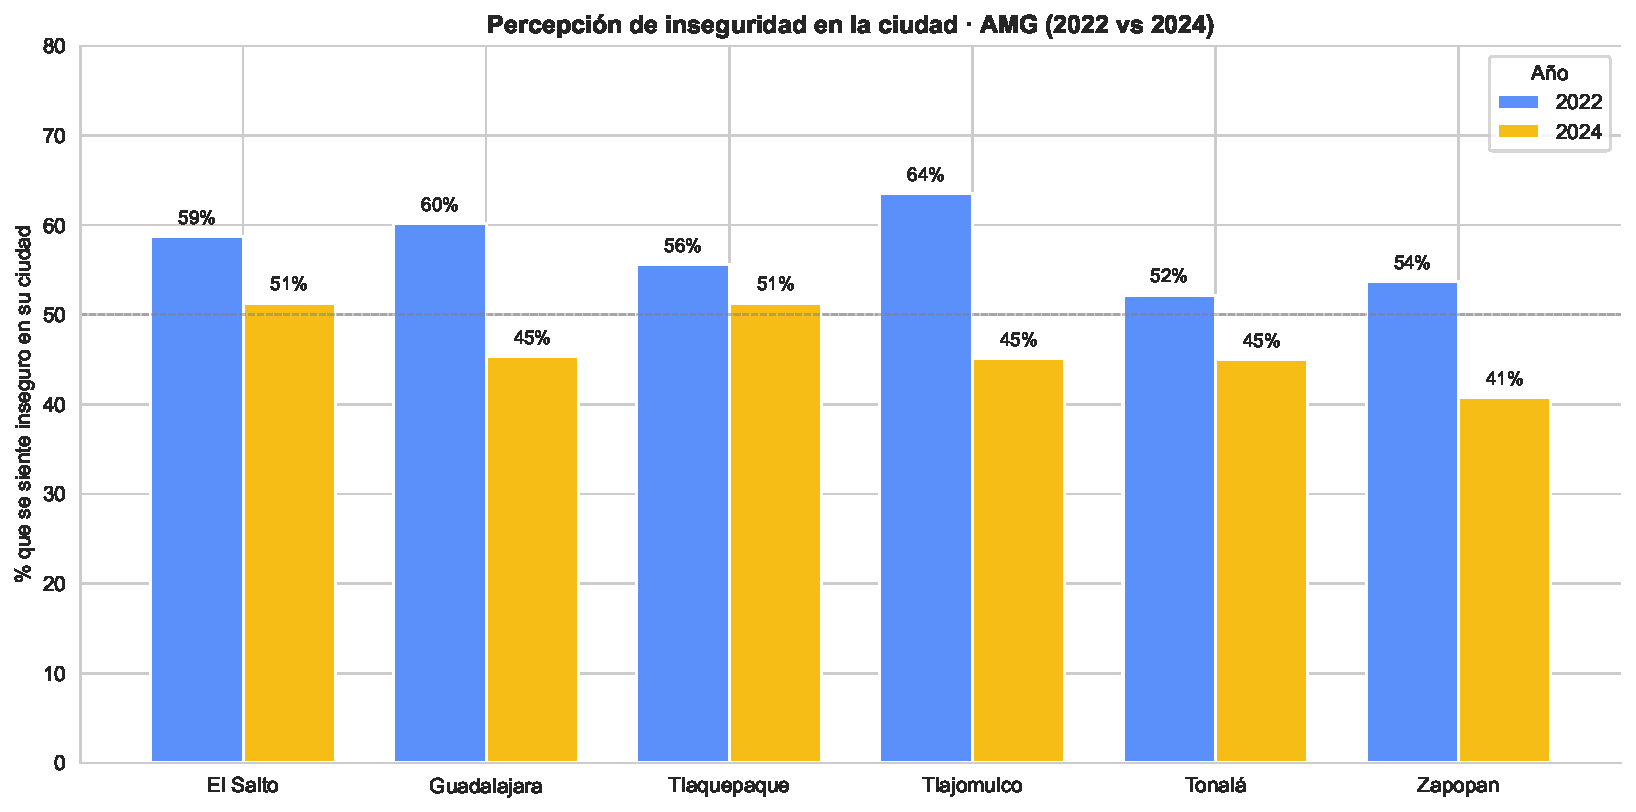
\includegraphics[width=\columnwidth]{figuras/fig01_percepcion_por_municipio.pdf}
  \caption{Percepción de inseguridad en la ciudad por municipio del AMG
  (JCV 2022 vs 2024). Elaboración propia con datos de [1], [2].}
  \label{fig:percepcion}
\end{figure}

\subsection{Proporción de víctimas que no denunciaron}

La proporción de víctimas que declaró no haber denunciado disminuyó en
el conjunto del AMG, de 65.1\% en 2022 a 59.2\% en 2024. En Zapopan
también descendió, de 73.8\% a 68.7\%, aunque permaneció por encima del
valor metropolitano en ambos años. El comportamiento no fue uniforme:
entre 2022 y 2024 el indicador aumentó en Tlajomulco y Tonalá
(Tabla~\ref{tab:cifra_negra}). Estos valores describen únicamente la no
denuncia declarada y no la cifra negra completa definida por INEGI.

\begin{table}[H]
  \centering
  \caption{Víctimas que declararon no haber denunciado, por municipio
  del AMG, 2022 y 2024 (\%). Indicador parcial asociado a la cifra negra.}
  \label{tab:cifra_negra}
  \small
  \begin{tabular}{lrrr}
    \toprule
    Municipio & 2022 & 2024 & $\Delta$ (pp) \\
    \midrule
    Total AMG     & 65.1 & 59.2 & $-5.9$ \\
    El Salto      & 66.7 & 62.0 & $-4.7$ \\
    Guadalajara   & 60.6 & 46.5 & $-14.1$ \\
    Tlaquepaque   & 64.8 & 58.5 & $-6.3$ \\
    Tlajomulco    & 59.1 & 64.8 & $+5.7$ \\
    Tonalá        & 68.7 & 70.4 & $+1.7$ \\
    Zapopan       & 73.8 & 68.7 & $-5.1$ \\
    \bottomrule
  \end{tabular}
\end{table}

\subsection{Confianza en la policía}

La desconfianza total en la policía (categoría ``nada'') bajó de 54.4\%
a 42.5\% en el AMG, en Zapopan la reducción fue mayor (57.5\% $\to$
34.1\%), aunque uno de cada tres habitantes sigue declarando
desconfianza total (Fig.~\ref{fig:confianza}).

\begin{figure}[H]
  \centering
  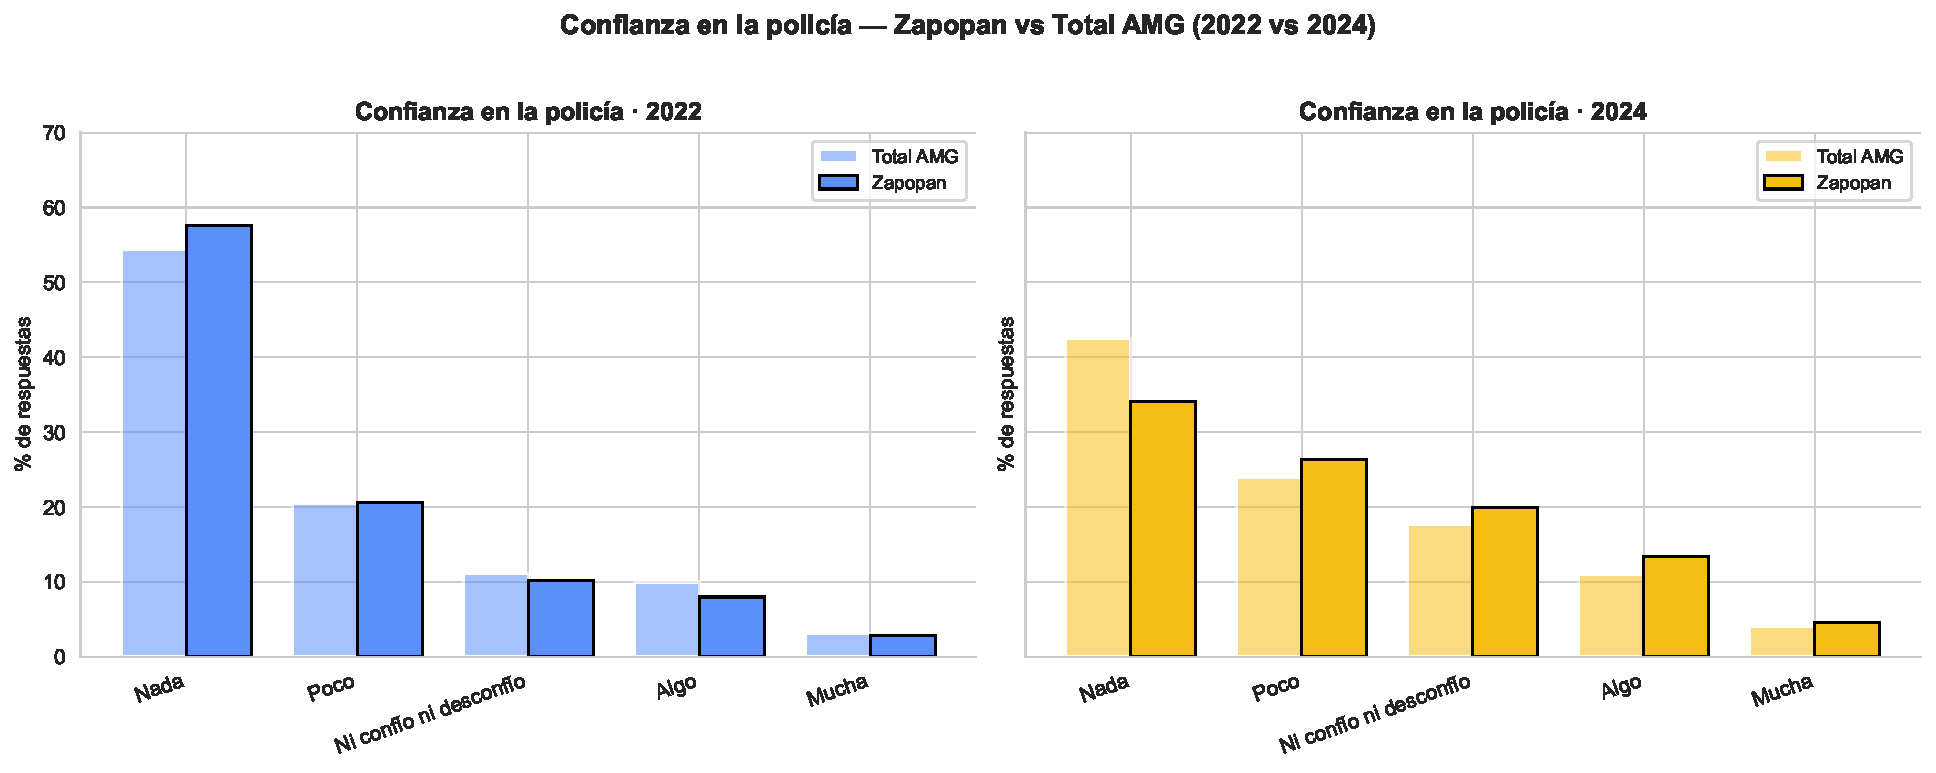
\includegraphics[width=\columnwidth]{figuras/fig02_confianza_policia.pdf}
  \caption{Distribución de la confianza en la policía en Zapopan y el
  total del AMG (2022 vs 2024).}
  \label{fig:confianza}
\end{figure}

\subsection{Panorama de las tres métricas}

La Fig.~\ref{fig:heatmap} sintetiza las tres métricas clave. La
percepción de inseguridad, la no denuncia y la respuesta ``nada'' de
confianza policial disminuyeron en Zapopan entre ambos levantamientos.
Sin embargo, la proporción de no denuncia continuó siendo elevada.
Estas tendencias agregadas no permiten establecer por sí solas una
relación entre percepción, confianza y decisión individual de denunciar.

\begin{figure*}[htbp]
  \centering
  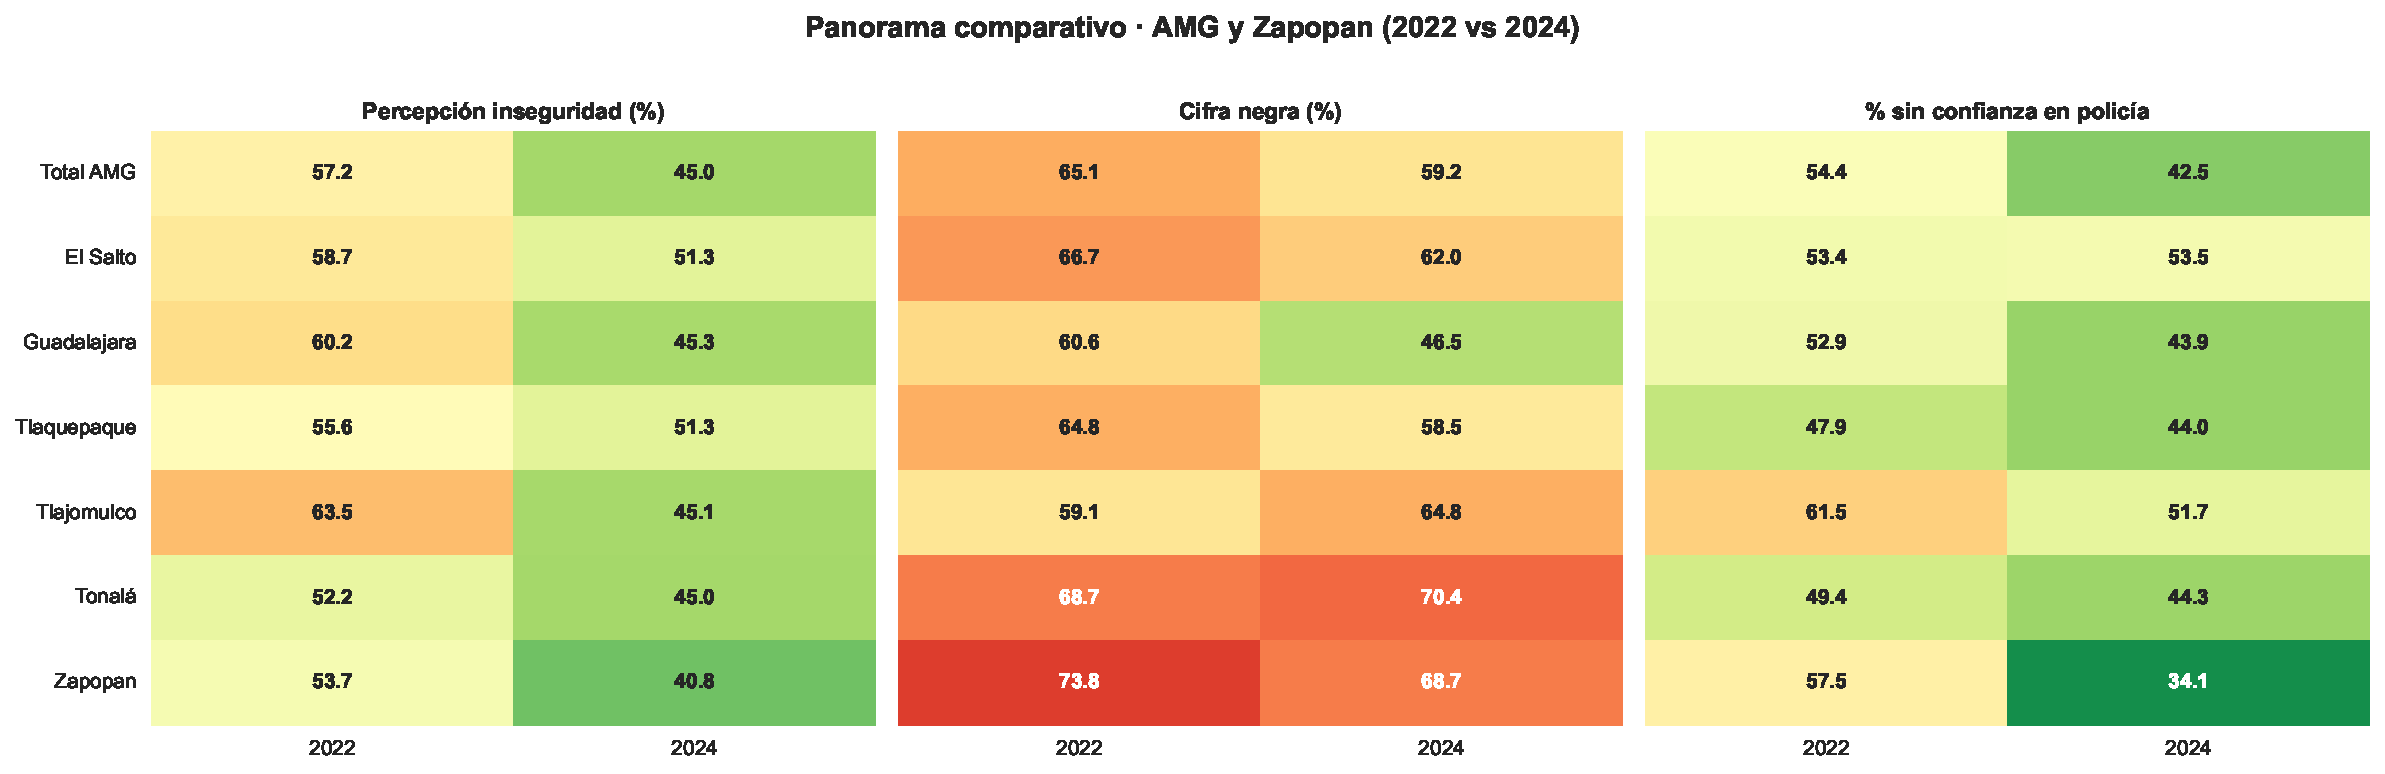
\includegraphics[width=\textwidth]{figuras/fig03_heatmap_3metricas.pdf}
  \caption{Comparación de percepción, proporción de no denuncia
  (indicador parcial asociado a la cifra negra) y respuestas ``nada''
  de confianza en la policía por municipio (2022 y 2024). Los tonos
  rojos representan valores más altos.}
  \label{fig:heatmap}
\end{figure*}

\subsection{Brechas sociodemográficas}

En 2024, la proporción de mujeres que manifestó sentirse poco o nada
segura fue de 49.8\%, frente a 39.9\% entre los hombres, una brecha de
9.9 pp. Por edad, el valor más alto correspondió al grupo de 45--59 años
(51.3\%), seguido por el de 60 años o más (48.5\%). Estas diferencias
son descriptivas y no se sometieron a pruebas de significancia
(Fig.~\ref{fig:brechas}).

\begin{figure}[H]
  \centering
  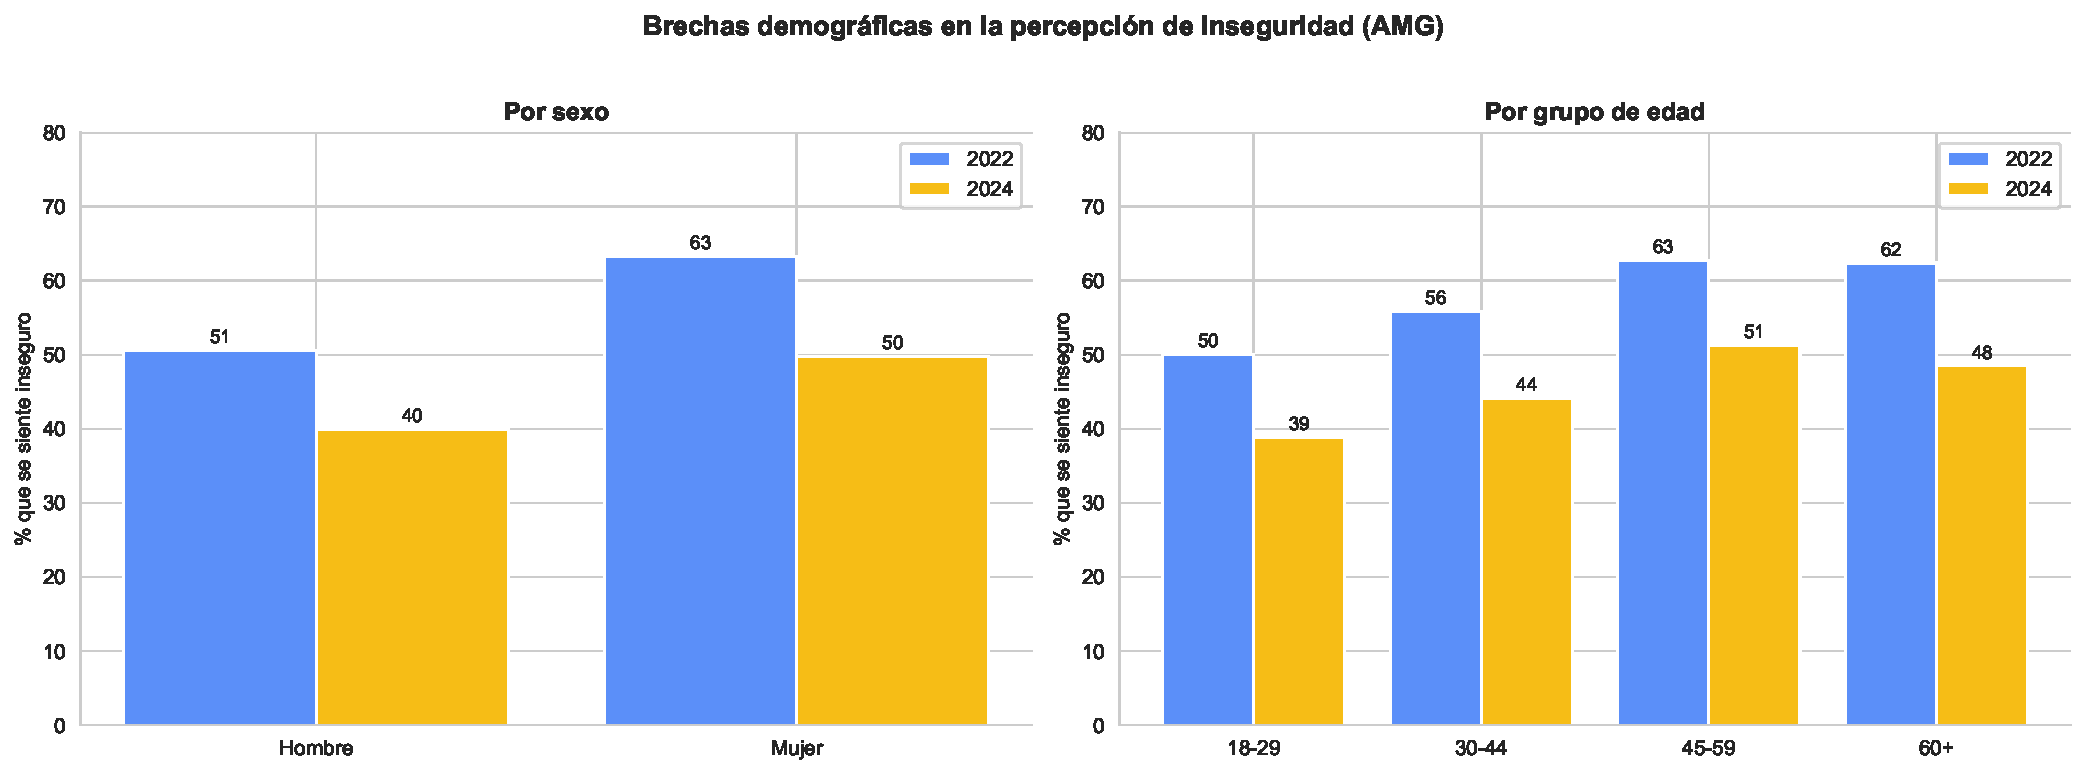
\includegraphics[width=\columnwidth]{figuras/fig04_brechas_sexo_edad.pdf}
  \caption{Percepción de inseguridad por sexo y grupo de edad (AMG,
  JCV 2022 vs 2024).}
  \label{fig:brechas}
\end{figure}

\subsection{Razones para no denunciar}

Los motivos declarados muestran que la decisión de no denunciar no se
atribuye a una sola causa. En 2024, la categoría conjunta ``No sirve /
Pérdida de tiempo'' concentró 40.2\% de las respuestas válidas entre
quienes no denunciaron; le siguieron ``Desconfianza en la autoridad''
(17.1\%) y ``Delito de poca importancia'' (15.9\%). En 2022, las tres
categorías equivalentes sumaban 23.2\%, 22.1\% y 10.5\%,
respectivamente. La desconfianza explícita en la autoridad aumentó de
10.5\% a 17.1\% entre ambos levantamientos (6.6 pp). La categoría de
utilidad o tiempo debe interpretarse con cautela: en 2022 sus motivos
aparecen separados y en 2024 se presentan agrupados. Otros motivos
incluyen falta de pruebas, temor al agresor o a una extorsión,
desconocimiento del lugar para denunciar, actitud negativa de la
autoridad y trámites largos o difíciles [1], [2]. En conjunto, las
respuestas apuntan a barreras percibidas de eficacia, tiempo y
confianza, además de obstáculos de información, protección y acceso;
no permiten determinar por sí solas el peso causal de cada barrera
(Fig.~\ref{fig:razones}).

\begin{figure}[H]
  \centering
  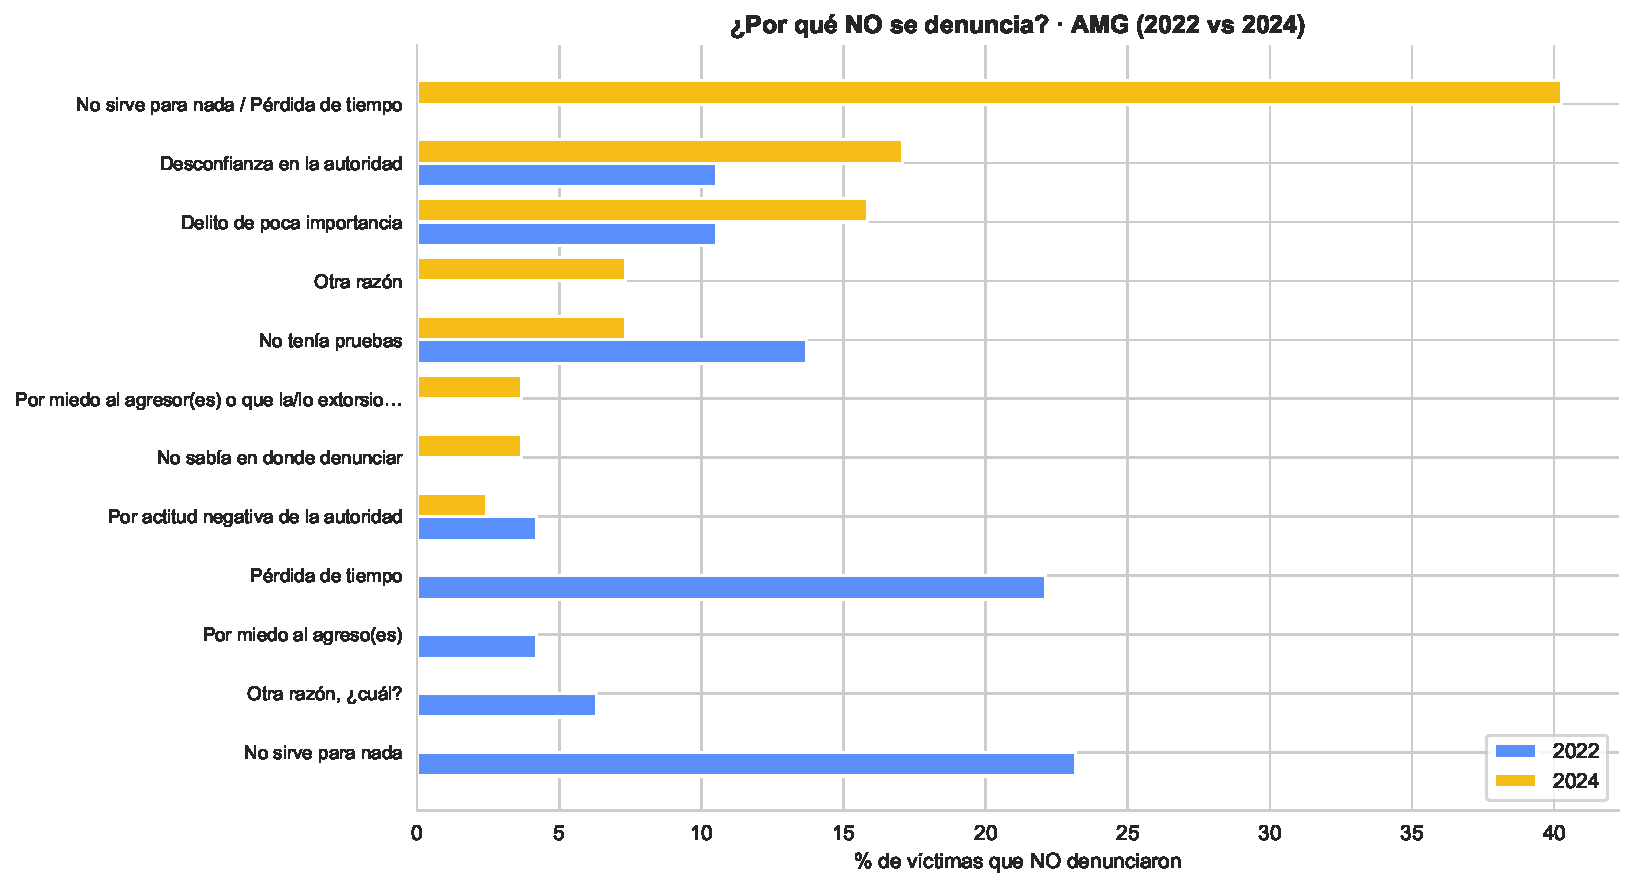
\includegraphics[width=\columnwidth]{figuras/fig05_razones_no_denuncia.pdf}
  \caption{Motivos declarados para no denunciar en el AMG, como
  porcentaje de respuestas válidas entre quienes no denunciaron.
  ``No sirve / Pérdida de tiempo'' reúne categorías separadas en 2022
  (23.2\% y 22.1\%) y agrupadas en 2024 (40.2\%). ``Desconfianza en la
  autoridad'' aumentó de 10.5\% a 17.1\% (6.6 pp); ``Delito de poca
  importancia'' pasó de 10.5\% a 15.9\%. La ausencia de una barra no
  equivale necesariamente a cero.}
  \label{fig:razones}
\end{figure}

\subsection{Validación externa: JCV vs ENSU}

Los resultados de JCV de 2024 y de la ENSU de marzo de 2026 ofrecen una
referencia contextual, no una comparación directa. En los cuatro
municipios con datos para ambos instrumentos, las diferencias van de
11.2 pp en San Pedro Tlaquepaque a 44.9 pp en Guadalajara. La distancia
puede relacionarse con diferencias de periodo, diseño muestral y
formulación de los reactivos, además de cambios en el contexto. Por
tanto, no debe atribuirse a una sola causa ni interpretarse como una
validación de una serie respecto de la otra (Fig.~\ref{fig:jcv_ensu}).

\begin{figure}[H]
  \centering
  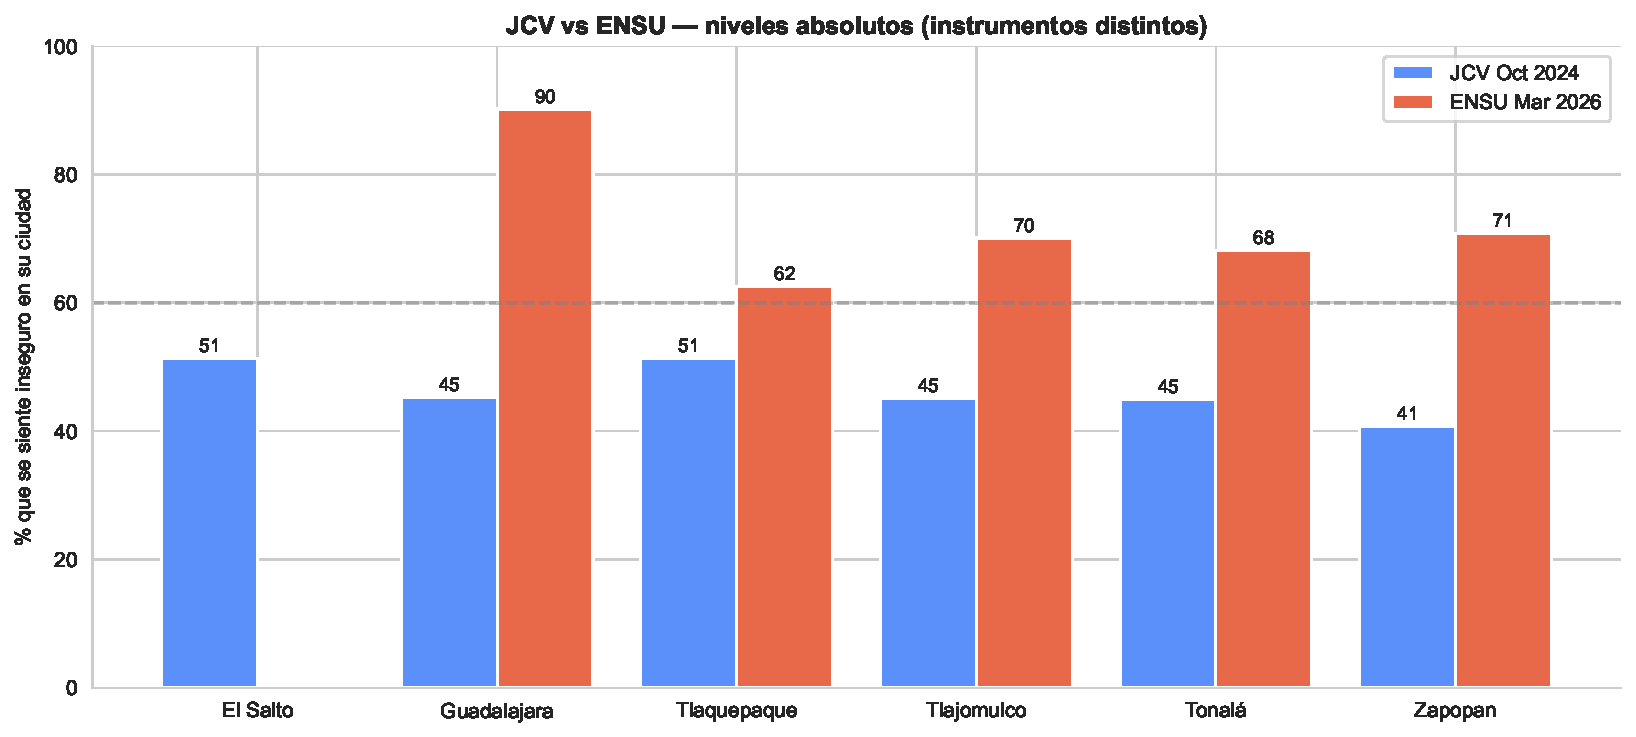
\includegraphics[width=\columnwidth]{figuras/fig06_jcv_vs_ensu.pdf}
  \caption{Comparación de los niveles de percepción entre JCV
  (octubre 2024) y ENSU (marzo 2026). Instrumentos distintos: no son
  series comparables punto a punto.}
  \label{fig:jcv_ensu}
\end{figure}

\subsection{Percepción e incidencia registrada en Zapopan}

La percepción de inseguridad y las carpetas de investigación miden
dimensiones distintas: la primera es una valoración subjetiva; la
segunda, un registro administrativo que depende de los hechos
denunciados y de su procesamiento. En Zapopan, la percepción de JCV
disminuyó de 53.7\% en 2022 a 40.8\% en 2024, mientras que la tasa
referida de carpetas pasó de 1\,493 a 1\,492 por cada 100\,000
habitantes (Fig.~\ref{fig:carpetas}). La estabilidad de la tasa entre
2022 y 2024 no demuestra por sí sola ni una reducción de los delitos
ocurridos ni una mayor eficacia institucional. Con solo dos
observaciones anuales y sin una serie independiente de incidencia, la
comparación es contextual, no concluyente. Se incluye como referencia,
no como validación de la encuesta ni estimación de la cifra negra [1],
[2], [5], [10].

\begin{figure}[H]
  \centering
  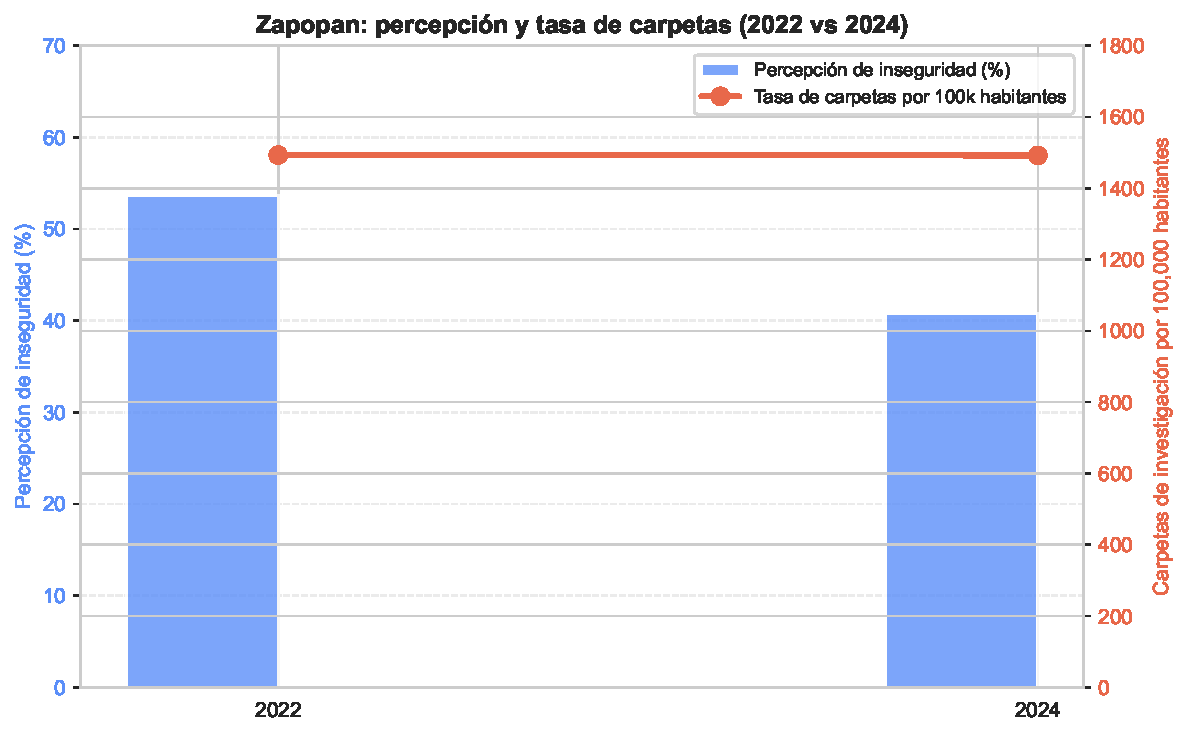
\includegraphics[width=\columnwidth]{figuras/fig07_percepcion_vs_carpetas_zapopan.pdf}
  \caption{Percepción de inseguridad (JCV) y tasa de carpetas por
  100\,000 habitantes (SESNSP, consultada vía MunicipioData) en
  Zapopan, 2022 y 2024. Percepción y carpetas miden cosas distintas:
  la estabilidad de los registros no demuestra por sí sola ni menos
  delitos ni más eficacia [1], [2], [5], [10].}
  \label{fig:carpetas}
\end{figure}

\subsection{Referencias externas sobre motivos institucionales}

La Fig.~\ref{fig:causas_autoridad} agrega contexto sobre los obstáculos
institucionales reportados en Jalisco: pérdida de tiempo (35\%) y
trámites largos o difíciles (11\%) con referencia a ENVIPE 2023, y
desconfianza en la autoridad (12.3\%) con referencia a Jalisco en 2021
[8], [9]. No son porcentajes de JCV ni observaciones de un mismo año.
Por ello, la figura no debe leerse como una tendencia temporal ni como
una comparación directa entre motivos; complementa, con cautela, las
barreras reportadas por las personas encuestadas por JCV en la
Fig.~\ref{fig:razones}.

\begin{figure}[H]
  \centering
  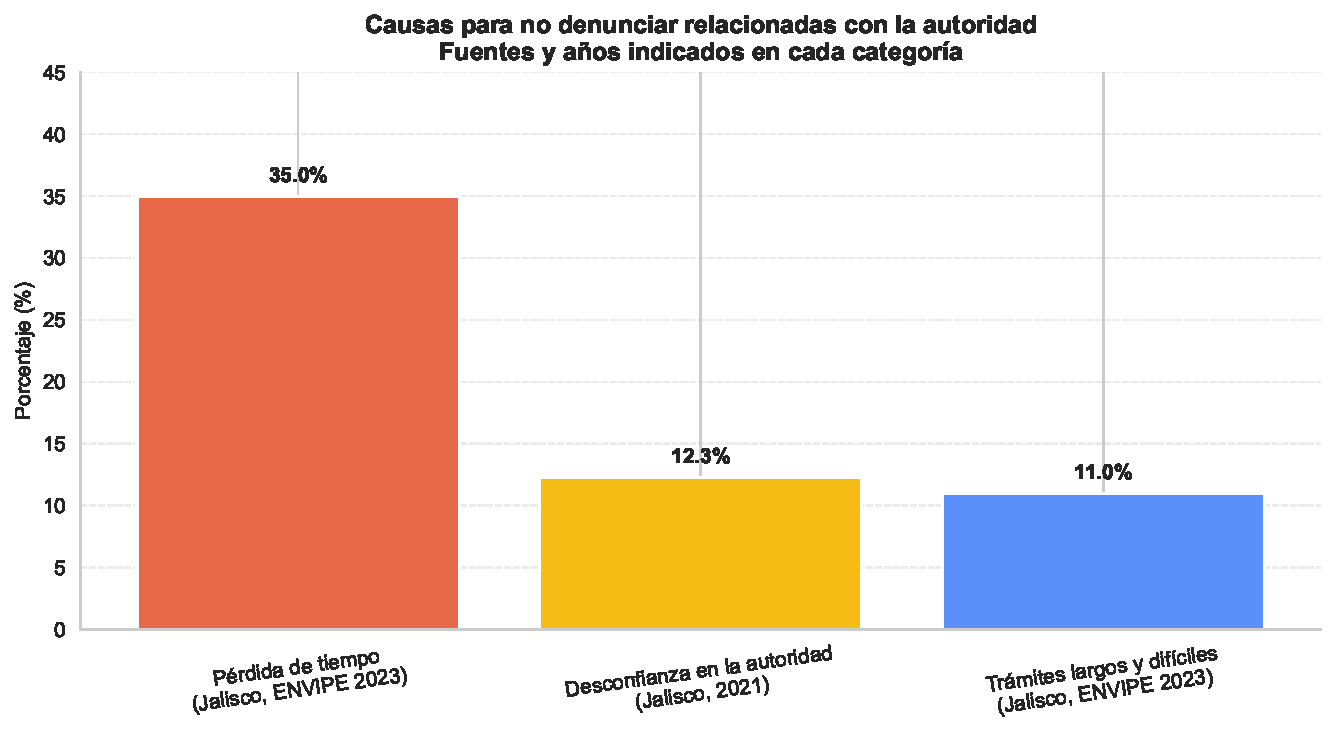
\includegraphics[width=\columnwidth]{figuras/fig08_causas_no_denuncia.pdf}
  \caption{Motivos relacionados con la autoridad para no denunciar en
  Jalisco, según fuentes disponibles: pérdida de tiempo (35\%,
  ENVIPE 2023) y trámites largos o difíciles (11\%, ENVIPE 2023);
  desconfianza en la autoridad (12.3\%, referencia de Jalisco 2021).
  Los años y fuentes difieren, por lo que los porcentajes no forman
  una serie homogénea ni deben sumarse. Se incluyen únicamente como
  contexto externo a los datos de JCV [8], [9].}
  \label{fig:causas_autoridad}
\end{figure}

\section{Discusión}

Los resultados muestran cambios simultáneos, pero no idénticos, en los
indicadores. Entre 2022 y 2024 disminuyeron la percepción de inseguridad
(12.2 pp en el AMG y 12.9 pp en Zapopan) y la proporción de víctimas que
no denunciaron (5.9 pp y 5.1 pp, respectivamente). Esta última, no
obstante, permaneció en 59.2\% para el AMG y 68.7\% para Zapopan; además,
aumentó en Tlajomulco y Tonalá. La respuesta ``nada'' de confianza en la
policía también disminuyó en el agregado, mientras que la desconfianza
en la autoridad como motivo declarado para no denunciar aumentó 6.6 pp.
Este contraste se refiere a indicadores y denominadores distintos; no
demuestra que la confianza policial determine la conducta de denuncia.

Los motivos declarados ayudan a matizar la lectura de la no denuncia. En
2024, cuatro de cada diez respuestas válidas se concentraron en la
percepción de que denunciar no sirve o implica pérdida de tiempo. Esto
es consistente con la teoría de la elección racional y los costes de
transacción de la denuncia (sección II-A): si la utilidad esperada del
trámite es baja y el costo de tiempo es alto, la abstención puede ser
una decisión racional; sin embargo, la encuesta no permite distinguir
entre ambas explicaciones, pues las categorías aparecen agrupadas. La
desconfianza en la autoridad constituye otro motivo relevante, junto con
la poca importancia atribuida al delito, la falta de pruebas, el temor y
las barreras de información o acceso. Por ello, la confianza
institucional es parte de la explicación declarada, pero no la única.

Los datos descriptivos no permiten confirmar una ``crisis estructural''
ni atribuir la reducción de la percepción a cambios en la incidencia
delictiva. No obstante, el patrón observado —reducción moderada de la
percepción y de la no denuncia, junto con persistencia de motivos
atribuibles a la autoridad y aumento de la desconfianza declarada— es
\textit{consistente} con los marcos teóricos de la elección racional y
del círculo vicioso entre impunidad y desconfianza (secciones II-A y
II-B). La consistencia teórica no equivale a evidencia causal; se
requiere triangulación con datos de carpetas de investigación y con la
cifra negra estimada por ENVIPE para avanzar en esa dirección.

\subsection{La ``baja oficial'' de delitos frente a la percepción real}

Un punto metodológico central es distinguir entre delitos ocurridos y
delitos registrados. Las estadísticas del SESNSP contabilizan carpetas
de investigación, no la cantidad total de delitos [5]. En Zapopan, la
tasa referida para este análisis se mantuvo prácticamente estable:
1\,493 por cada 100\,000 habitantes en 2022 y 1\,492 en 2024
(Fig.~\ref{fig:carpetas}). Al mismo tiempo, la percepción de inseguridad
de JCV descendió de 53.7\% a 40.8\%. Esta divergencia entre indicadores
puede motivar la hipótesis de un \textit{espejismo estadístico}: la
estabilidad o reducción de los registros administrativos no demuestra,
por sí sola, que hayan disminuido los delitos ocurridos ni que haya
aumentado la eficacia institucional. Una baja en la denuncia puede
contribuir a reducir los registros y dejar hechos fuera de las
estadísticas oficiales.

Sin embargo, los datos de este estudio no muestran un aumento general
de la abstención de denunciar entre 2022 y 2024: la proporción de
víctimas que declaró no denunciar bajó en el AMG y en Zapopan, aunque
subió en Tlajomulco y Tonalá. Además, solo se dispone de dos
observaciones anuales de la tasa de carpetas y no se analiza aquí una
serie de incidencia delictiva independiente. Por ello, la comparación
no prueba que la tasa estable de carpetas sea producto de una menor
denuncia ni permite afirmar una ``falsa métrica'' de eficacia. El
espejismo estadístico se plantea como una advertencia sobre los límites
de los registros administrativos, no como una explicación causal de
los cambios observados. Para distinguir entre cambios en victimización,
denuncia y procesamiento institucional se requiere triangular registros
de carpetas con encuestas de victimización y estimaciones de cifra negra
de ENVIPE [4], [5], [7].

Como implicación práctica, los motivos reportados justifican evaluar
medidas que reduzcan costos de tiempo y complejidad, faciliten la
orientación sobre dónde denunciar, mejoren la comunicación sobre el
seguimiento de los casos y ofrezcan condiciones de atención seguras a
las víctimas. Estas son líneas de acción derivadas de las barreras
declaradas; su efectividad requiere evaluación específica.

\subsection{Limitaciones}

El estudio utiliza tablas cruzadas agregadas, por lo que no permite
analizar trayectorias individuales, intervalos de confianza ni
significancia estadística. Las categorías de motivos de no denuncia
tampoco son idénticas entre 2022 y 2024: por ejemplo, ``No sirve para
nada'' y ``Pérdida de tiempo'' aparecen separadas en 2022 y agrupadas en
2024. Además, el indicador de no denuncia no incluye los delitos
denunciados sin inicio de carpeta, por lo que no equivale a la cifra
negra completa de ENVIPE. Finalmente, JCV y ENSU difieren en periodo,
diseño y formulación de preguntas; sus niveles no son directamente
intercambiables. Los resultados deben leerse como una descripción
comparativa de las categorías disponibles, no como evidencia causal.

\section{Conclusiones}

Entre 2022 y 2024, la percepción de inseguridad disminuyó 12.2 pp en el
AMG y 12.9 pp en Zapopan. La proporción de víctimas que no denunció
también bajó, en 5.9 pp y 5.1 pp, respectivamente, aunque en 2024
continuó en 59.2\% para el AMG y 68.7\% para Zapopan. La desconfianza en
la autoridad como motivo declarado para no denunciar aumentó 6.6 pp.
Estos datos muestran que la reducción de la no denuncia y la persistencia
de barreras declaradas pueden coexistir; no bastan para afirmar una
crisis estructural ni para establecer una relación causal entre
percepción, confianza y denuncia. En conjunto, los hallazgos son
\textit{consistentes con} la hipótesis de una crisis de confianza
institucional estructural, pero no la demuestran: la evidencia es
descriptiva y se limita a dos levantamientos.

Los motivos más mencionados en 2024 —la percepción de inutilidad o el
costo de tiempo, la desconfianza en la autoridad y la poca importancia
atribuida al delito— señalan ámbitos que las instituciones pueden
examinar: simplificación de trámites, orientación accesible, seguimiento
transparente de denuncias y atención que tome en cuenta la seguridad de
las víctimas. La brecha de género observada en la percepción (9.9 pp en
2024) también justifica que futuras evaluaciones desagreguen resultados
por sexo y otras características sociodemográficas.

\section{Trabajos futuros}

\subsection{Recomendaciones de política pública}

\subsubsection{Reducción de los costos de transacción de la denuncia}

En 2024, ``No sirve / Pérdida de tiempo'' concentró 40.2\% de las
respuestas válidas sobre motivos para no denunciar en JCV; este
porcentaje no corresponde al total de víctimas, sino a la distribución
renormalizada de motivos (Fig.~\ref{fig:razones}). Se propone evaluar
una Ventanilla Digital Unificada e interoperable que permita iniciar y,
cuando el procedimiento lo autorice, ratificar una denuncia mediante
firma electrónica, además de consultar su seguimiento remoto. La
simplificación de requisitos y la reducción de esperas buscan disminuir
el costo de tiempo y trámite descrito por las personas encuestadas, en
concordancia con la teoría de la elección racional y los costes de
transacción (sección II-A). Los tiempos de atención podrían evaluarse
antes y después de su implementación; no se presupone que el trámite
pueda reducirse a una duración específica. Deben contemplarse
accesibilidad para quienes tienen conectividad limitada y alternativas
de atención presencial.

\subsubsection{Transparencia activa y trazabilidad de los casos}

La desconfianza en la autoridad como motivo para no denunciar aumentó
de 10.5\% en 2022 a 17.1\% en 2024, dentro de la distribución válida de
motivos (Fig.~\ref{fig:razones}). Se propone evaluar un portal público
e interactivo, que podría integrarse con MIDE Zapopan si existe
viabilidad técnica e institucional. El portal reportaría, con
metodología y denominadores explícitos, indicadores agregados de avance,
judicialización y resolución de carpetas por tipo de delito y ámbito
territorial. La desagregación por colonia requeriría suprimir o agrupar
celdas con pocos casos para proteger a víctimas y evitar su
identificación. La publicación periódica de resultados verificables
puede contribuir a distinguir cambios en las denuncias de cambios en la
incidencia delictiva, cuestión relacionada con el ``espejismo
estadístico'' discutido en la sección V-A. El número de carpetas no debe
presentarse como un conteo completo de los delitos ocurridos.

\subsubsection{Evaluación de protocolos de atención a víctimas}

También podría evaluarse la capacitación del personal y la aplicación
de protocolos de atención a víctimas con perspectiva de género,
orientados a atender la desconfianza declarada en la autoridad (17.1\%
en JCV 2024; Fig.~\ref{fig:razones}) y a prevenir la revictimización
durante la denuncia. La evaluación tendría que definir indicadores de
trato y seguridad percibida, además de mecanismos de seguimiento y
retroalimentación de las personas usuarias.

\subsection{Mejora metodológica: análisis de microdatos}

Las tablas cruzadas agregadas no permiten reconstruir la variabilidad
individual ni estimar intervalos de confianza o pruebas de
significancia para los contrastes con la información disponible. Como
siguiente paso, se propone solicitar y analizar los microdatos
individuales de JCV y, cuando estén disponibles y sus variables sean
comparables, los de ENVIPE. Se requerirían los cuestionarios y la
documentación del diseño muestral, así como ponderadores, estratos y
conglomerados para calcular estimaciones e incertidumbre acordes con
cada encuesta. Esto permitiría examinar conjuntamente nivel
socioeconómico, edad, sexo y características de la victimización, sin
asumir que las preguntas de ambos instrumentos son equivalentes. Las
inferencias causales seguirían requiriendo un diseño de investigación
apropiado.

\subsection{Línea de investigación: decisión individual de denunciar}

Con microdatos adecuados podría estimarse un modelo de regresión
logística binaria para estudiar qué variables se asocian con que una
víctima denuncie. Entre las variables de interés están la confianza
institucional, la percepción de impunidad, el tipo de delito, el tiempo
o costo percibido del trámite, el nivel socioeconómico, la edad, el sexo
y los ingresos, siempre que estén medidos con calidad suficiente. Un
modelo multinivel (persona, colonia y municipio) sería pertinente solo
si el tamaño de muestra, la estructura de los datos y las claves
geográficas lo permiten. Este análisis conectaría el marco de elección
racional con la evidencia empírica, pero sus resultados describirían
asociaciones y no demostrarían causalidad por sí solos.

\section*{Agradecimientos}

Producto derivado del proyecto de investigación ``La percepción de
inseguridad en AMG'', apoyado por la Universidad de Guadalajara. Se
agradece a Jalisco Cómo Vamos y al IIEG por la disponibilidad de sus
datos abiertos.

% REFERENCIAS (formato IEEE)
\begingroup
\small
\renewcommand{\section}[2]{}
\begin{thebibliography}{99}

\bibitem{jcvv2024}
Jalisco Cómo Vamos, \textit{IX Encuesta de Percepción sobre Calidad de
Vida, octubre 2024. Bases de datos de tablas cruzadas.} Guadalajara,
México: JCV, 2024.

\bibitem{jcvv2022}
Jalisco Cómo Vamos, \textit{VIII Encuesta de Percepción sobre Calidad de
Vida, 2022. Bases de datos de tablas cruzadas.} Guadalajara, México:
JCV, 2022.

\bibitem{ensu2026}
INEGI, \textit{Encuesta Nacional de Seguridad Pública Urbana (ENSU).
Principales resultados para Jalisco, marzo 2026.} Guadalajara, México:
IIEG, 2026. [En línea]. Disponible en:
\url{https://iieg.gob.mx/ns/?page_id=25306}

\bibitem{envipe2024}
INEGI, \textit{Encuesta Nacional de Victimización y Percepción sobre
Seguridad Pública (ENVIPE) 2024.} Aguascalientes, México: INEGI, 2024.

\bibitem{sesnsp2024}
Secretariado Ejecutivo del Sistema Nacional de Seguridad Pública
(SESNSP), \textit{Incidencia delictiva del fuero común. Datos abiertos.}
Ciudad de México, México: SESNSP, 2024. [En línea]. Disponible en:
\url{https://www.gob.mx/sesnsp/acciones-y-programas/datos-abiertos-de-incidencia-delictiva}

\bibitem{becker1968}
G. S. Becker, ``Crime and punishment: An economic approach,''
\textit{Journal of Political Economy}, vol. 76, no. 2, pp. 169--217,
1968.

\bibitem{iieg2024}
Instituto de Información Estadística y Geográfica de Jalisco (IIEG),
\textit{Cifra negra del delito en Jalisco, 2023.} Guadalajara, México:
IIEG, 2024. [En línea]. Disponible en:
\url{https://iieg.gob.mx/ns/wp-content/uploads/2024/09/Ficha-Cifra-negra-2024.pdf}

\bibitem{envipe2023}
INEGI, \textit{Encuesta Nacional de Victimización y Percepción sobre
Seguridad Pública (ENVIPE) 2023.} Aguascalientes, México: INEGI, 2023.
[En línea]. Disponible en:
\url{https://www.inegi.org.mx/programas/envipe/2023/}

\bibitem{envipe2021}
INEGI, \textit{Encuesta Nacional de Victimización y Percepción sobre
Seguridad Pública (ENVIPE) 2021.} Aguascalientes, México: INEGI, 2021.
[En línea]. Disponible en:
\url{https://www.inegi.org.mx/programas/envipe/2021/}

\bibitem{municipiodata}
MunicipioData, \textit{Portal de datos municipales: incidencia delictiva
en Zapopan.} [En línea]. Disponible en:
\url{https://municipiodata.com/}

\bibitem{percepcion_amg} J. Martínez, \textit{La percepción de inseguridad en AMG.} 
[En línea]. Disponible en: 
\url{https://github.com/josue-mtz/La_percepcion_de_inseguridad_en_AMG}


\end{thebibliography}
\endgroup

\end{document}